\documentclass[14pt]{matmex-diploma-custom}

\begin{document}

\filltitle{ru}{
    chair              = {Кафедра информатики},
    title              = {Разработка системы автоматического анализа новостных публикаций на финансовом рынке},
    %   coursework - Курсовая работа
    %   diploma - Диплом специалиста
    %   master - Диплом магистра
    %   bachelor - Диплом бакалавра
    type               = {bachelor},
    position           = {студента},
    group              = 13.Б09-мм,
    author             = {Зернов Алексей Викторович},
    supervisorPosition = {к.\,ф.-м.\,н., доцент},
    supervisor         = {Григорьев Д.\,А.},
    reviewerPosition   = {д.\,т.\,н., декан},
    reviewer           = {Мусаев А.\,А.},
%   chairHeadPosition  = {д.\,ф.-м.\,н., профессор},
%   chairHead          = {Новиков Б.\,А.},
    university         = {Санкт-Петербургский Государственный Университет},
    faculty            = {Математико-механический факультет},
    city               = {Санкт-Петербург},
    year               = {2017}	
}
\filltitle{en}{
    chair              = {Computer Science Department},
    title              = {Development of the automatic analysis system of a financial market's news publications},
    type               = {bachelor},
    position           = {student},
    group              = {13.Б09-мм},
    author             = {Zernov Alexey Viktorovich},
    supervisorPosition = {Sc.\,C., associate professor},
    supervisor         = {Grigoryev D.\,A.},
    reviewerPosition   = {Sc.\,D., dean},
    reviewer           = {Musaev A.\,A.},
%   chairHeadPosition  = {professor},
%   chairHead          = {Boris Novikov},
    faculty            = {Faculty of Mathematics and Mechanics},
    city               = {Saint-Petersburg},
    year               = {2017}
}

\maketitle

\tableofcontents

\clearpage\section*{Введение}

Не смотря на то, что с каждым годом происходит увеличение доли цифровой информации по отношению к бумажной, все равно остается проблема работы с этими данными. Дело в том, что большинство такой информации является неструктурированной, а следовательно на ее обработку требуется достаточно много времени и человеческих ресурсов. Целью данной работы является написание программы, позволяющей уменьшенить объем временных затрат на изучение большого потока новостных публикаций в тех случаях, когда необходимо оценить изменение стоимости акций определенной компании по связанным с ней новостям.

В работе будут рассмотрены основные определения, связанные с финансовым рынком (Раздел~\ref{sec:finance}); базовая теория, касаемая интеллектуального анализа текста (Раздел~\ref{sec:analysis}); существующие решения (Раздел~\ref{sec:overview}) и представлен результат работы в виде программы, осуществляющей анализ новостных публикаций с возможностью последующего предсказания изменения стоимости акций (Раздел~\ref{sec:program}).

\clearpage\section{Финансовый рынок}

\label{sec:finance}

В данном разделе будет представлен краткий обзор основных терминов, связанных с самим финансовым рынком, его структурой и основными участниками. Более подробная информация может быть получена в книге \cite{book:financial_market}.

\subsection{Определение}

В более общем виде \textbf{финансовый рынок}~--- совокупность экономических связей его участников, касающихся создания, поддержания и обращения капитала. Финансовый рынок является довольно абстрактным термином, и под ним часто подразумеваются более конкретные: рынок купонных и бескупонных облигаций, рынок акций (или фондовый рынок) или валютный рынок. Не смотря на выделение составляющих, каждая из них является частью единого механизма, в котором финансы перемещаются между каждым из конкретных рынков.

Каждый из финансовых рынков является рынком посредников между начальными владельцами финансов и их конечными пользователями. Если рынок основывается на финансах как на капитале, он называется фондовым рынком, и именно в этой роли выступает как составная часть всего финансового рынка.

В России финансовые рынки имеют следующие критерии, влияющие на их деятельность:

\begin{itemize}
\item Инвестиции в экономику страны
\item Международные рынки, влиние тенденций глобализации
\item Современные компьютерные технологии
\item Уровень комьютерной и информационной развитости участников рынков
\end{itemize}

\subsection{Структура}

Финансовый рынок может быть:

\begin{itemize}
\item Первичным или вторичным
\item Организованным или неорганизованным
\item Биржевым или внебиржевым
\item Традиционным или компьютеризированным
\item Кассовым или срочным
\end{itemize}

\textbf{Первичный рынок} обеспечивает выход ценных бумаг в оборот, это своеобразное <<производство>> ценных бумаг. На \textbf{вторичном рынке} в обороте находятся уже выпущенные ранее ценные бумаги. Вторичный рынок представляет из себя совокупность всех операций с данными ценными бумагами, в результате которых они переходят от одних владельцев к другим.

\textbf{Организованный рынок} отличается от \textbf{неорганизованного рынка} тем, что в первом имеются единые для всех участников рынка правила, за соблюдением которых следят организаторы. В неорганизованном рынке соблюдение единых правил для всех участников рынка не гарантируется.

\textbf{Биржевой рынок}~--- такой рынок, на котором в качестве инструмента торговли используется аукцион. Руководителем же является некоторый специалист, например, NYSE\footnote{New York Stock Exchange~--- Нью-Йоркская фондовая биржа} или AMEX\footnote{American Stock Exchange - Американская фондовая биржа}. На \textbf{внебиржевых рынках} торги организуются при помощи электронных систем.

\textbf{Срочный рынок} чаще всего подразумевает отложенное исполнение сделки, в отличие от \textbf{кассового рынка}, когда сделки исполняются сразу. Обычно традиционные ценные бумаги (акции, облигации) идут в оборот на кассовых рынках, а контракты на производные инструменты рынка ценных бумаг~--- на срочных.

\subsection{Участники}

\textbf{Участники} рынка ценных бумаг~--- это физические лица или компании, которые продают или приобретают ценные бумаги, обеспечивают их оборот или расчеты по ним. 

Основными участниками рынка выступают \textbf{эмитенты}, выпускающие акции или облигации, с помощью которых привлекают финансирование, а также размещающие свободные на данный момент денежные средства. Эмитентами могут быть: государство, субъекты государства или коммерческие предприятия. Целью эмитентов на первичном рынке является размещение запланированного транша по максимальной цене.

\textbf{Инвестор}~--- лицо, заинтересованное во вложении капитала в ценные бумаги. Целью инвесторов является как можно более выгодная покупка ценных бумаг максимально перспективных компаний.

\clearpage\section{Интеллектуальный анализ текста}

\label{sec:analysis}

В настоящее время можно заметить увеличение роли компьютеров в жизни каждого человека. Инорфмация хранится преимущественно в цифровом виде, что значительно упрощает поиск или работу с ней. Но не смотря на это, многие данные все равно остаются довольно трудными для анализа, не смотря на оцифрованный вид, из-за чего можно подразделить из на следующие формы:

\begin{itemize}
\item Структурированные данные
\item Частично структурированные данные
\item Неструктурированные данные
\end{itemize}

Хорошим примером \textbf{структурированных данных} могут являться базы данных. \textbf{Частично структурированные данные}~--- это электронные письма, разнообразные файлы на языках разметок (HTML, XML и другие).

Если работа со структурированными или частично структурированными данными достаточно детерминированная, то \textbf{неструктурированные данные} представляют наибольший интерес в этом вопросе. Около 80\% корпоративных данных находится именно в неструктурированном формате, в котором сложно проводить поиск или извлекать необходимую информацию. Для этого нужны специфические методы и алгоритмы обработки. И поскольку самая популярная форма хранения информации~--- это текст, интеллектуальный анализ текста (text mining) является более важным процессом, нежели интеллектуальный анализ данных (data mining).

Интеллектуальный анализ текста стоит на пересечении дисциплин и включает в себя: обработку web-данных, информационный поиск, компьютерную лингвистику и обработку естественного языка.

\subsection{Процесс интеллектуального анализа текста}

Концепция интеллектуального анализа текста представлена в \cite{article:text_mining}. В интеллектуальном анализе текста можно выделить два основных этапа (Рис.~\ref{img:text_mining}):

\begin{itemize}
\item Фильтрация текста
\item Извлечение знаний
\end{itemize}

\begin{figure}[h]
\centering
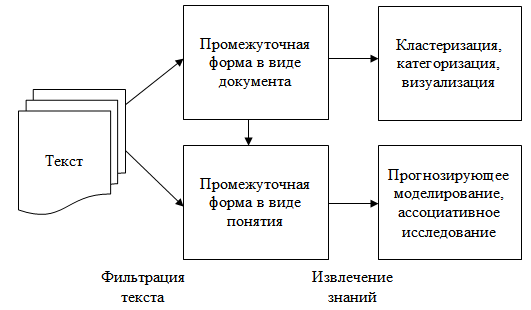
\includegraphics[width=0.7\textwidth]{img/text_mining}
\caption{Общий процесс интеллектуального анализа текста}
\label{img:text_mining}
\end{figure}

\textbf{Фильтрация} (или очистка) преобразует исходный текстовый документ в некоторое промежуточное представление. \textbf{Извлечение знаний}, в свою очередь, получает полезную информацию (знания) или некоторые шаблоны уже из промежуточного представления. Промежуточное представление может быть как структурированным, так и частично структурированным. Также оно может быть как новым текстовым документом, так понятием, в котором составляющие являются данными или наборами данных из какой-либо предметной области.

Анализ промежуточного представления в виде документов выдает образцы и связи между всеми документами. 

Анализ промежуточного представления в виде понятий выдает образцы и связи между объектами или другими понятиями.

Примеры задач анализа промежуточного представления в виде документов: \emph{кластеризация}, \emph{визуализация} и \emph{категоризация документов}; примеры задач анализа промежуточного представления в виде понятий: \emph{прогнозирующее моделирование} и \emph{ассоциативное исследование}.

Промежуточное представление в виде документа может быть преобразовано в промежуточное представление в виде понятия путем выделения релевантной информации, которая относится к необходимым объектам из какой-либо предметной области. Отсюда вытекает то, что промежуточное представление чаще не зависит от конкретное предметной области. К примеру, новостные потоки при фильтрации текста преобразуются в промежуточные представления в виде документов, соответствующим определенным статьям. Затем, в зависимости от поставленных задач визуализации или навигации, каждый документ (статья) проходит обработку знаний. Для извлечения же знаний в определенной предметной области промежуточное представление в виде документа может быть преобразовано в промежуточное представление в виде понятия в соответствии с необходимыми требованиями. К примеру, можно извлечь информацию, касающуюся определенного товара или услуги из промежуточного представления в виде документа и сформировать базу данных товаров или услуг для предоставления знаний о них.

\subsubsection{Предварительная обработка текста}

Предварительная обработка включает в себя:

\begin{enumerate}
\item Токенизацию
\item Удаление <<стоп-слов>>
\item Определение происхождения слов
\end{enumerate}

\paragraph{Токенизация} 

Сначала текст разделяется на отдельные слова, освобождаясь от пробелов и знаков препинания.

\paragraph{Удаление <<стоп-слов>>}

На этом этапе происходит избавление от <<ненужных>> конструкций текста. Это могут быть HTML или XML теги, предлоги, артикли и прочее.

\paragraph{Происхождения слов} 

Представляет из себя выявление корней определенных слов. Порой эта обработка бывает более грубой и выделяются, например, только своеобразные основы (обрубаются окончания или приставки).

\subsubsection{Преобразование текста}

Текстовый документ состоит из слов и информации об их происхождении. Два основных подхода представления документа: <<мешок слов>> (<<bag-of-words>>) и векторные пространства слов.

\subsubsection{Поиск признаков}

Под признаками можно понимать переменные. То есть в результате этого шага отбирается подмножество наиболее значимых признаков для их дальнейшего применения при построении моделей. Убираются, например, признаки, которые избыточны или не несут никакой информации.

\subsubsection{Методы анализа текста}

На данном шаге начинается построение модели с использованием разных методов, таких как кластеризация, классификация, информационный поиск и других. Данные методы распознавания данных также подходят и для интеллектуального анализа текста.

\subsubsection{Интерпретация и оценка}

На последнем шаге (в зависимости от того, что требуется) проводится анализ результатов.

\subsection{Области применения интеллектуального анализа текста}

Как уже упоминалось выше, интеллектуальный анализ текста стоит на пересечении разных дисциплин и включает в себя: извлечение информации, информационный поиск, обработку естественного языка и интеллектуальный анализ данных.

\subsubsection{Извлечение информации}

В процессе извлечения информации автоматически извлекается структурированная информация из неструктурированных данных. С помощью распознавания образов данная система определяет, например, где имена людей, где названия компаний, а где местоположение. То есть в документах происходит поиск предопределенных последовательностей. Подобное решение позволяет получить элементы, подходящие для использования в базах данных для дальнейшего хранения, анализа или обработки.

\subsubsection{Информационный поиск}

В данной задаче используются методы, используемые для хранения, представления и доступа к информации, которая преимущественно представлена в виде текстовых документов (а также новостных лент или книг), которые могут быть получены по запросу пользователя. Это своего рода расширение поиска по документам, позволяющее сужать набор документов, имеющих отношение к запросу пользователя. Эти системы значительно сокращают время, необходимое для поиска необходимой информации. Наиболее известными системами информационного поиска являются поисковые системы Google.

\subsubsection{Обработка естественного языка}

Данная задача представляет из себя самую активную проблему в области искусственного интеллекта. Цель: исследовать естественный язык так, чтобы у компьютеров была возможность понимать языки, подобные тем, что используют для общения люди. Обработка естественного языка включает в себя распознавание и генерацию, которые отвечают за такие способности компьютера как <<читать>> и <<говорить>> на естественном языке соответственно. Подобные системы включают в себя проверку грамматики, лексические, синтаксические и семантические анализаторы.

\subsubsection{Интеллектуальный анализ данных}

Данные задачи относятся к поиску знаний или релевантной информации в большом объеме данных. Система пытается обнаружить правила (статистически) и образцы (автоматически) от данных. Подобные системы имеют возможность предсказания, основываясь на <<опыте>>, полученном в результате исследования.

\clearpage\section{Обзор существующих инструментов}

\label{sec:overview}

В данном разделе будут рассмотрены основные инструменты, представленные в виде библиотек или отдельных сервисов. Внимание уделено в основном инструментам, работающим с русским языком.

\subsection{Natural Language Toolkit}

NLTK\cite{tools:nltk} является пакетом библиотек и программ для разработки программ на Python, работающих с естественным языком. Сопровождается обширной документацией, а также книгой\footnote{\url{http://www.nltk.org/book/}}, объясняющей основные концепции проблем, для решения которых предназначен данный пакет.

Данный пакет подходит для таких областей как компьютерная лингвистика, эмпирическая лингвистика, когнитивистика, искусственный интеллект, информационный поиск и машинное обучение. NLTK используется преимущественно в качестве учебного пособия, индивидуального обучения или прототипирования и создания систем, ориентированных на научно-исследовательскую деятельность.

NLTK~--- свободное программное обеспечение, то есть доступное бесплатно.

\subsection{Pymorphy2}

Pymorphy2\cite{tools:pymorphy2} написан на языке Python и имеет следующие возможности:

\begin{itemize}

\item Приведение слова к нормальной форме

\item Ставить слово в нужную форму

\item Возвращать грамматическую информацию о слове

\end{itemize}

Распространяется pymorphy2 под лицензией MIT\footnote{\url{https://opensource.org/licenses/MIT}}, если используется в научной работе.

\subsection{Томита-парсер}

Томита-парсер\footnote{\url{https://tech.yandex.ru/tomita/}} способен извлекать структурированные данные из текстов на естественном языке. Как и почти во всех инструментах, рассматриваемых в данном разделе, Томита-парсер ориентирован преимущественно на русскоязычные тексты. В нем используются контекстно-свободные грамматики и словари ключевых слов. Код проекта\footnote{\url{https://github.com/yandex/tomita-parser/}} (написан на C и C++) находится в свободном доступе.

\subsection{Яндекс.Спеллер}

Яндекс.Спеллер\footnote{\url{https://tech.yandex.ru/speller/}} выполняет задачу проверки орфографии в текстах на английском, русском и украинском языках. Для этого используется орфографический словарь. К тому же, предоставлен набор API методов (для JavaScript) для реализации данной проверки разработчиками сайтов или приложений.

\subsection{OntosMiner}

OntosMiner\footnote{\url{http://my-eventos.com/solution/ontosminer/}} является решением компании Eventos\footnote{\url{http://my-eventos.com/solution/ontosminer/}}, занимающейся в большей степени разработкой продуктов в области лингвистического анализа текстовой информации, кластеризацией и классификацией информации. Конкретно OntosMiner является целой комплексной системой, дающей возможность распознавания связей между сущностями в текстах на естественной языке. Также, она позволяет определять общую тональность текста.

\clearpage\section{Программная часть}

\label{sec:program}

В результате работы была написана программа\footnote{\url{https://github.com/Zernov/diploma/tree/master/src}}, позволяющая автоматически анализировать новостные публикации сайта \url{mfd.ru}.

\subsection{Описание}

Программа способна выполнять следующие функции:

\begin{itemize}
\item Загружать заданное количество последних новостных публикаций определенной компании
\item Загружать данные о котировках определенной компании за заданный промежуток времени
\item Формировать и обучать рекурентную нейронную сеть по заданным данным
\item Предсказывать изменение цены по заданной новостной публикации
\end{itemize}

На вход программы подается название компании, выступающей в роли эмитента, количество новостей, начальная и конечные даты, в течение которых необходимо получить изменение изменения цен. В результате работы программы получаются следующие файлы:

\begin{itemize}
\item \texttt{news/company.csv}~--- скаченные новости в формате csv с двумя колонками: дата и текст
\item \texttt{stocks/company.csv}~--- скаченные котировки в формате csv с двумя колонками: дата и стоимость акций
\item \texttt{stems/company.csv}~--- обработанные новости в формате, аналогичном \texttt{news/company.csv}
\item \texttt{connections/company.csv}~--- соединенные новости и котировки в формате csv с тремя колонками: дата, обработанный текст и изменение акции (положительное или отрицательное)
\end{itemize}

\subsection{Используемые инструменты}

Выбор инструментов основывался на тех задачах, которые нужно было решать в процессе написания программы. Исходя из поставленной задачи можно выделить следующие подзадачи:

\begin{itemize}
\item Загрузка данных с интернет-ресурсов, для чего необходима работа с web-запросами
\item Преобразование содержимого web-страниц, для чего нужны инструменты преобразования содержимого HTML-файлов
\item Преобразование текстовых документов в более пригодный для обучения вид
\item Обучение рекурентной нейронной сети, для чего необходимы соответствующие инструменты
\end{itemize}

В связи с подзадачами был выбран язык программирования Python версии 3.6.0 и библиотеки \texttt{urllib}\footnote{\url{https://docs.python.org/3/library/urllib.html}} (работа с web-запросами) версии 1.21.1, \texttt{bs4}\footnote{\url{https://www.crummy.com/software/BeautifulSoup/bs4/doc/}} (обработка html-файлов) версии 4.6.0, \texttt{nltk}\footnote{\url{http://www.nltk.org/}}\cite{tools:nltk} (преобразование текстовых документов) версии 3.2.2 и \texttt{keras}\footnote{\url{https://keras.io}}\cite{tools:keras} (работа с рекурентными нейронными сетями) версии 2.0.3. Возможность написания всех программных модулей на одном языке упрощает разработку и поддержку, что было еще одним преимуществом.

\subsection{Структура программы}

Всего в программе присутствует 6 основных файлов (модулей), каждый из которых отвечает за свою часть работы (Рис.~\ref{img:class}).

\begin{itemize}
\item \texttt{news\_getter.py} отвечает за скачивание новостей с сайта \url{mfd.ru}, за запись новостей в файл и за чтение новостей из файла
\item \texttt{stock\_getter.py} отвечает за загрузку котировок с сайта \url{finam.ru}, за запись котировок в файл и за чтение котировок из файла
\item \texttt{connector.py} является вспомогательным модулем, ответственным за объединение новостей и подсчет изменения котировок за соответствующие даты
\item \texttt{stemmer.py} выполняет небольшую задачу по выделению основ слов, чтобы избежать излишнего увеличения числа переменных при обучении
\item И наконец, все перечисленные выше файлы подключатся в основной (\texttt{main.py}), который выполняет последовательно необходимые действия и имеет два метода: обучение нейронной сети по данным и предсказание изменений по заданному набору новостей
\end{itemize}

\begin{figure}[h]
\centering
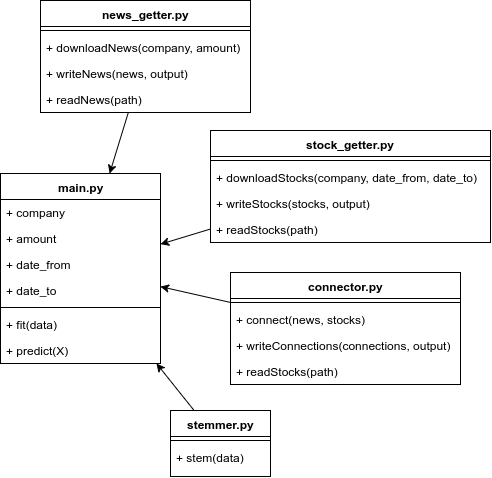
\includegraphics[width=0.7\textwidth]{img/class}
\caption{Структура программы}
\label{img:class}
\end{figure}

\subsection{Работа программы}

Работу программы можно разбить на два основных этапа: предварительная обработка и построение модели. Во время предварительной обработки происходит загрузка и преобразование данных (включая стемминг и удаление <<стоп-слов>>). Во время построения модели выделяются и строятся требуемые слои рекурентной нейронной сети.

\subsubsection{Предварительная обработка}

Изначально необходимо получить требуемые данные: тексты новостей и котировок. В случае добавления и/или изменения новостных источников или сайтов, позволяющих загрузить данные о котировках, затрагивается только единственный метод в соответствующем модуле.

\paragraph{Экспорт новостей}

В случае экспорта новостей информационным источником выступал сайт \url{mfd.ru}. В методе \texttt{downloadNews} (Приложение~\ref{app:downloadNews}), который находится в модуле \texttt{news\_getter.py}, имеются два входных параметра: название компании и количество требуемых новостей. Название компании преобразуется в идентификатор эмитента соответствующей компании на сайте \url{mfd.ru}, после чего строятся адреса последних новостей в требуемом количестве, и начинается загрузка. Подобное решение было принято в связи с тем, что новостная лента может обновляться во время загрузки большого количества данных, требуемых для обучения, и в результате загрузки мы получим дублирование некоторых новостей. Факт долгой загрузки большого объема данных так же создает проблему возможных сбоев при загрузке. Она была решена отловом различных HTTP-ошибок с остановкой запросов на некоторое время и последующим возобновлением загрузки. После загрузки новости к результатам добавлялась очередная пара, состоящая из даты и текста новости. Результат экспорта возвращался в основную программу для дальнейших действий с ним (записи в файл или непосредственной обработки).

\paragraph{Экспорт котировок}

В случае экспорта котировок данные получались с сайта \url{finam.ru}, на котором имеется возможность с помощью HTTP-запроса получить информацию по котировкам определенной компании. Метод, отвечающий за это, называется \texttt{downloadStocks} (Приложение~\ref{app:downloadStocks}) и находится в модуле \texttt{stock\_getter.py}. На вход он принимает три параметра: название компании и границы дат, между которыми необходимо получить информацию. Название компании позволяет определить идентификатор эмитента соответствующей компании и ее код~--- параметры в адресе запроса. В данной работе единицей измерения интервала между стоимостями котировок являлся один день. Из нескольких цен, предоставленных в результате экспорта (цена на момент открытия торгов, цена на момент закрытия торгов, максимальная цена за время торгов и минимальная цена за время торгов) бралась единственная~--- цена на момент открытия торгов. Далее именно разница между ценами на момент открытия торгов в два разных дня станет оценкой новостей, опубликованных за этот промежуток времени. Результатом экспорта является набор пар, состоящих из даты и цены на момент открытия торгов в этот день, и он возвращается в основную программу для дальнейших действий (записи в файл или непосредственной обработки).

\paragraph{Преобразование данных}

Преобразование данных тоже можно разбить на две части: обработка текста и соединение новостей с соответствующими котировками по датам. Первую часть выполняет метод \texttt{stem} (Приложение~\ref{app:stem}) модуля \texttt{stemmer.py}, принимающий на вход необработанные новости. При обработке текста новости в первую очередь убираются цифры, знаки пунктуации и латинские буквы (в связи с их небольшим количеством). Затем каждое слово в тексте проходит операцию стемминга, то есть выделения основы слова для избавления от чрезмерного дублирования похожих слов в словаре. В этом же методе происходит <<склейка>> новостей одного дня в единую новость этого же дня. Результатом обработки текста является набор, содержащий даты с соответствующими <<склеенными>> новостями, содержащими лишь основы слов без знаков пунктуации, цифр и латинских букв. После этого этапа происходит создание подходящего набора данных для обучения, содержащего новости и соответствующие им оценки (в простейшем случае 0, если последовали отрицательные изменения и 1, если последовали положительные изменения). За эту задачу отвечает метод \texttt{connect} (Приложение~\ref{app:connect}) в соответствующем модуле \texttt{connector.py}, принимающий на вход новости и котировки. Изначально выделяется пересечение множеств дат из обоих наборов данных (количество этих дат и определяет размер набора данных для обучения). В случае отсутствия информации о котировках в день, в который была опубликована новость, она <<склеивается>> с предыдущими (как в обработке текста). Затем для каждой новости вычисляется ее оценка: 0, если цена акций к следующей новости упала, и 1 в противном случае. Результатом соединения является набор троек: дата, новость, оценка. После отработки метода, его результат возвращается в основную программу, где текст проходит предварительную обработку с помощью \texttt{Tokenizer}~--- класса, позволяющего индексировать все слова данного множества текстов, превратив их тем самым в наборы чисел, каждое из которых указывает на соответствующее слово в словаре.

\subsubsection{Построение модели}

Как уже было сказано ранее, на основе полученных данных программа обучает рекурентную нейронную сеть (RNN). Рекурентая нейронная сеть отличается от обычной наличием памяти. Однако в первоначальной ее модели память имеет небольшой объем~--- несколько элементов. В связи с этим было принято решение использовать метод LSTM \cite{tools:lstm}, имеющий более объемную память и более высокую скорость обучения по сравнению с другими моделями рекурентных нейронных сетей. Как видно из кода (Приложение~\ref{app:fit}), в модели присутствуют слои: Embending, LSTM, Dropout, Dense и Activation (Рис.~\ref{img:layers}). Рассмотрим подробнее некоторые из них.

\begin{figure}[h]
\centering
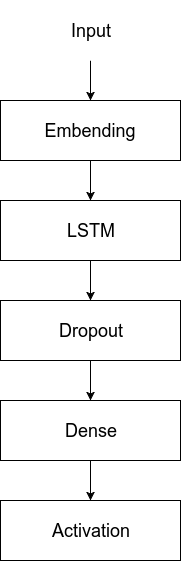
\includegraphics[width=0.2\textwidth]{img/layers}
\caption{Слои модели рекурентной нейронной сети}
\label{img:layers}
\end{figure}

\paragraph{Embending}

Этот слой преобразует индексы слов в вектора заданной размерности. Задача этого слоя~--- придать семантическое значение индексам, чтобы похожие слова имели близкие векторы.

\paragraph{LSTM}

Схема работы LSTM подробно описана в работе \cite{tools:lstm}.

\paragraph{Dropout}

Схема работы Dropout подробно описана в работе \cite{tools:dropout}. Задачей этого метода является предотвращение переобучения: на каждом шаге обнуляется $pn$ компонент входного вектора, где $p$~--- параметр Dropout, а $n$~--- длина вектора.

\paragraph{Dense}

В данном слое задаются параметры регуляризации, позволяющие уменьшить риск переобучения.

\paragraph{Activation}

В конце вычисляется активационная сигмоидальная функция, принимающая значение из полуинтервала $[0;1)$, интерпретируемая как вероятность изменения акций в положительную сторону.

\clearpage\section{Результаты}



\clearpage\section*{Заключение}

Будет добавлено после финальных экспериментов

\setmonofont[Mapping=tex-text]{CMU Typewriter Text}
\bibliographystyle{ugost2008ls}
\bibliography{diploma}

\begin{appendices}

\section{Исходный код метода downloadNews}

\label{app:downloadNews}

\begin{footnotesize}
\begin{lstlisting}[language=Python]
def downloadNews(company, amount):
 domain = 'http://mfd.ru'
 news_dates = []
 news = []
 news_count = 0
 if company == 'sberbank':
  company = '1'
 elif company == 'gazprom':
  company = '3'
 amount = int(amount)
 trs = getTrs(company, amount)
 total = len(trs)
 current = 0
 while current < total:
  try:
   td = trs[current].findAll('td')
   temp_date = td[0].getText().split(',')[0].strip()
   if temp_date == 'сегодня':
    today = datetime.date.today()
    item_date = today.strftime('%d/%m/%y')
   elif temp_date == 'вчера':
    yesterday = datetime.date.today() - datetime.timedelta(1)
    item_date = yesterday.strftime('%d/%m/%y')
   else:
    temp_date_split = temp_date.split('.')
    item_date = '{}/{}/{}'.format(str(temp_date_split[0]),
     str(temp_date_split[1]), str(temp_date_split[2][2:]))
    item_url = domain + td[1].find('a').get('href')
    item_bs = BeautifulSoup(urlopen(item_url), 'html.parser')
    item_content = item_bs.find('div', { 'class' : 'm-content' })
    item_data = item_content.findAll('p')
    item_string = ''
    for j in range(1, len(item_data) - 2):
     item_string += item_data[j].getText() + ' '
     item_string = item_string.strip()
     if item_string != '':
      news_dates.append(item_date)
      news.append(item_string)
      news_count += 1
     current += 1
     time.sleep(delay)
    except:
     time.sleep(delay_except)
 return news_dates[::-1], news[::-1], news_count
\end{lstlisting}
\end{footnotesize}

\section{Исходный код метода downloadStocks}

\label{app:downloadStocks}

\begin{footnotesize}
\begin{lstlisting}[language=Python]
def downloadStock(company, date_from, date_to):
 company = str(company)
 if company == 'sberbank':
  code = 'SBER'
  em = '3'
 elif company == 'gazprom':
  code = 'GAZP'
  em = '16842'
 dfs = date_from.split('/')
 df = dfs[0].lstrip('0')
 mf = str(int(dfs[1].lstrip('0')) - 1)
 yf = dfs[2]
 datef = dfs[0] + '.' + dfs[1] + '.' + dfs[2]
 dts = date_to.split('/')
 dt = dts[0].lstrip('0')
 mt = str(int(dts[1].lstrip('0')) - 1)
 yt = dts[2]
 datet = dts[0] + '.' + dts[1] + '.' + dts[2]
 cn = company
 url = 'http://export.finam.ru/stock.txt?market=1&em={}&code={}' +
    '&apply=0&df={}&mf={}&yf={}&from={}&dt={}&mt={}&yt={}&to={}' +
    '&p=8&f=stock_1&e=.txt&cn={}&dtf=4&tmf=3&MSOR=1&mstime=on' +
    '&mstimever=1&sep=1&sep2=1&datf=5&at=1'.format(em, code, 
       df, mf, yf, datef, dt, mt, yt, datet, cn)
 stocks_dates = []
 stocks = []
 stocks_count = 0
 data = urlopen(url).read().decode("utf-8").split('\r\n')
 for i in range(1, len(data) - 1):
  item_split = data[i].split(',')
  stocks_dates.append(item_split[0])
  stocks.append(item_split[2])
  stocks_count += 1
 return stocks_dates, stocks, stocks_count
\end{lstlisting}
\end{footnotesize}

\section{Исходный код метода stem}

\label{app:stem}

\begin{footnotesize}
\begin{lstlisting}[language=Python]
def stem(news_dates, news, news_count):
 stems_dates = []
 [stems_dates.append(date) for date in news_dates if date not in stems_dates]
 stems = []
 stems_count = len(stems_dates)
 i = 0
 j = 0
 while i < stems_count:
  stem = []
  while j < news_count and stems_dates[i] == news_dates[j]:
   words = text_to_word_sequence(news[j], filters = ''.join(punctuation) + 
     '–—01234567890abcdefghijklmnopqrstuvwxyz')
    for word in words:
     if word not in stemmer.stopwords and word != ' ':
      stem.append(stemmer.stem(word))
   j += 1
  i += 1
  stems.append(' '.join(stem))
 return stems_dates, stems, stems_count
\end{lstlisting}
\end{footnotesize}

\section{Исходный код метода connect}

\label{app:connect}

\begin{footnotesize}
\begin{lstlisting}[language=Python]
def connect(news_dates, news, news_count, stocks_dates, stocks, stocks_count):
 connections_dates = []
 for i in range(news_count):
  for j in range(stocks_count):
   if news_dates[i] == stocks_dates[j] and 
     news_dates[i] not in connections_dates:
    connections_dates.append(news_dates[i])
 connections_news = []
 connections_stocks = []
 connections_count = len(connections_dates)
 i = 0
 j = 0
 k = 0
 while connections_dates[i] != news_dates[j]:
  j += 1
 while connections_dates[i] != stocks_dates[k]:
  k += 1
 while i < connections_count - 1:
  connection_news = []
  while j < news_count and connections_dates[i + 1] != news_dates[j]:
   connection_news.append(news[j])
   j += 1
  connections_news.append(' '.join(connection_news))
  stocks_start = float(stocks[k])
  while k < stocks_count and connections_dates[i + 1] != stocks_dates[k]:
   k += 1
  stocks_end = float(stocks[k])
  connection_stocks = 1 if stocks_end > stocks_start else 0
  connections_stocks.append(connection_stocks)
  i += 1
 return connections_dates[:-1], connections_news, connections_stocks,
  connections_count - 1
\end{lstlisting}
\end{footnotesize}

\section{Исходный код метода fit}

\label{app:fit}

\begin{footnotesize}
\begin{lstlisting}[language=Python]
def fit(name):
 model = Sequential()
 model.add(Embedding(input_dim=num_words, output_dim=dimension))
 model.add(LSTM(units=dimension))
 model.add(Dropout(rate=dropout_rate))
 model.add(Dense(units=1, kernel_regularizer=l1_l2(l1=l1_rate, l2=l2_rate)))
 model.add(Activation(activation='sigmoid'))
 model.compile(optimizer=Adam(lr=l_rate), loss=binary_crossentropy,
   metrics=[binary_accuracy])
 hist = model.fit(training_X, training_y, batch_size=batch_size, 
   epochs=epochs, validation_split=validation_split)
 model.save(path + 'models/{}_model-{}.h5'.format(company, name))
 with open(path + 'models/{}_history-{}.txt'.format(company, name), 
   'w+', encoding='utf8') as temp:
  temp.write(str(hist.history))
 score = model.evaluate(testing_X, testing_y, batch_size=batch_size)
 with open(path + 'models/{}_score-{}.txt'.format(company, name), 
   'w+', encoding='utf8') as temp:
  temp.write(str(score))
\end{lstlisting}
\end{footnotesize}


\section{Результаты работы}

Будут добавлены после финальных экспериментов

\end{appendices}

\end{document}
